\paragraph{Aanroepen met variabelen}

Functies kunnen ook worden aangeroepen met variabelen als concrete waarden voor de parameters. Zo hebben we bijvoorbeeld de volgende functie:

\vspace*{-\baselineskip}\begin{verbatim}
void twice(text):
  print(text)
  print(text)
\end{verbatim}\vspace*{-\baselineskip}

Als we deze functie als volgt aanroepen:

\vspace*{-\baselineskip}\begin{verbatim}
fruits = "pineapple blueberry"
twice(fruits)
\end{verbatim}\vspace*{-\baselineskip}

dan krijg je twee keer de tekst \texttt{pineapple blueberry} op je scherm geprint. De waarde van de variabele \texttt{fruits}, dat is de string \texttt{"pineapple blueberry"}, wordt namelijk meegegeven aan de functie \texttt{twice}. Op de regel met \texttt{twice(fruits)} wordt de huidige waarde van fruits  ingevuld. Dit kan je je voorstellen alsof de regel veranderd wordt naar \texttt{twice("pineapple blueberry")}. Binnen de functie \texttt{twice} wordt de string \texttt{"pineapple blueberry"} toegewezen aan \texttt{text}. Daarna wordt die waarde geprint.

% Let er goed op dat een functie de waarde gebruikt die wordt meegegeven. Zo kan je buiten de functie een variabele hebben met dezelfde naam als een parameter van de functie. Bijvoorbeeld:
%
% \vspace*{-\baselineskip}\begin{verbatim}
% name = "david"
% void call(person):
%   print(person)
% call("sarah")
% \end{verbatim}\vspace*{-\baselineskip}
%
% Dit stukje code print \texttt{sarah}. Hoewel er buiten de functie de variabele \texttt{person} bestaat met de waarde \texttt{"david"}, wordt de functie aangeroepen met de string \texttt{"sarah"}. De waarde \texttt{"sarah"} wordt toegewezen aan de variabele \texttt{person}, en zo wordt uiteindelijk \texttt{sarah} geprint.

Ook bij het aanroepen van functies met variabelen maakt de volgorde van de parameters uit:

\vspace*{-\baselineskip}\begin{verbatim}
x = 10
y = 40
void minus(x, y):
  print(x - y)
minus(y, x)
\end{verbatim}\vspace*{-\baselineskip}

Omdat de waardes van de variabelen worden meegegeven aan de functie wordt hier \texttt{30} geprint en niet \texttt{-30}. Je kan de regel \texttt{minus(y, x)} vervangen door \texttt{minus(40, 10)}, ofwel de waardes van de variabelen \texttt{x} en \texttt{y} op dat moment. Binnen de functie wordt de waarde \texttt{40} aan de variabele \texttt{x} en de waarde \texttt{10} aan de variabele \texttt{y} toegewezen. Dan wordt er \texttt{print(x - y)} uitgevoerd, ofwel \texttt{print(40 - 10)}.

\paragraph{Traceren}

We voegen nu expliciet een element aan de trace toe: het vervangen van de waarden in de functieaanroep. Bij de startregel strepen we de variabelenamen door, en vervangen deze door de waarden die eerder toegekend zijn. (Hierbij letten we nog helemaal \emph{niet} op de functiedefinitie!)

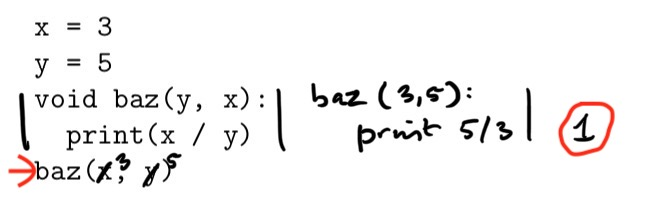
\includegraphics[width=.8\textwidth]{3-trace-varsparams.jpeg}

Nu de concrete waarden ingevuld zijn, kunnen we de trace verder opschrijven zoals in de vorige paragraaf.
